% % % % % % % % % % % % % % % % % % % % % 
% dbi.tex - Ian Huston
% $Id: dbi.tex,v 1.69 2009/12/07 16:43:29 ith Exp $
% % % % % % % % % % % % % % % % % % % % % 
% Redefine CVSRevision for this section
\renewcommand{\CVSrevision}{\version$Id: dbi.tex,v 1.69 2009/12/07 16:43:29 ith Exp $}

% % % % % % % % % % % % % % % % % % % % % % % % % % % % % % % % 
% =========================================================== %
% % % % % % % % % % % % % % % % % % % % % % % % % % % % % % % % 
\chapter{Observational Bounds on DBI Inflation}
\label{ch:dbi}
% % % % % % % % % % % % % % % % % % % % % % % % % % % % % % % % 
% =========================================================== %
% % % % % % % % % % % % % % % % % % % % % % % % % % % % % % % % 
% 
% 
% 
% % % % % % % % % % % % % % % % % % % % % % % % % % % % % % % % 
% =========================================================== %
% % % % % % % % % % % % % % % % % % % % % % % % % % % % % % % % 
\section{Introduction}
\label{sec:intro-dbi}
% % % % % % % % % % % % % % % % % % % % % % % % % % % % % % % % 
% =========================================================== %
% % % % % % % % % % % % % % % % % % % % % % % % % % % % % % % % 

In this chapter two bounds on the amplitude of primordial gravitational waves will be derived, which
severely challenge the standard
DBI inflationary scenario. By considering the field range of observable
inflation inside a warped throat, the tensor-scalar ratio $r$ will be
constrained to be less than $10^{-7}$. In contrast a lower bound of $r\gtrsim
0.005$ will be derived when the power spectrum of scalar perturbations has a red
spectral index. These clearly incompatible bounds can be relaxed by using a more
general form of the DBI action.

% 
The gravitational wave background generated in DBI 
inflation was initially investigated by Baumann \& McAllister (BM) 
\cite{bmpaper}. By exploiting a relationship due originally 
to Lyth \cite{lyth}, these authors derived a field-theoretic upper limit 
to the tensor amplitude and concluded that 
rather stringent conditions would need to be satisfied for these 
perturbations to be detectable.      
Moreover, the special case of 
DBI inflation driven by a quadratic potential is incompatible with the WMAP3 
data when this constraint is imposed \cite{bean}.  


Our aim in this chapter is to derive observational constraints on DBI inflation
that are 
insensitive to the details of the throat geometry and the inflaton potential. 
In general, there are two realisations of the scenario, 
which are referred to as the ultra-violet (UV) and infra-red (IR) 
versions. These are characterised respectively by whether the brane is 
moving towards or away from the tip of the throat. 
We focus initially on the UV scenario 
and derive an upper bound on 
the gravitational wave amplitude in terms of observable 
parameters. This limit arises by considering 
the variation of the inflaton field during the era when 
observable scales cross the Hubble radius, and 
we find in general that the tensor-scalar ratio must satisfy 
$r \lesssim 10^{-7}$. This 
is below the projected sensitivity of future CMB
polarisation 
experiments \cite{Baumann:2008aq,vpj}. 

On the other hand, the WMAP5 data 
favours a red perturbation spectrum, with 
$n_s<1$, when  
the scalar spectral index is effectively constant \cite{Komatsu:2008hk}. 
For models which generate such a spectrum, 
we identify a corresponding lower limit on the 
tensor modes such that $r \gtrsim 0.1 (1-n_s)$. 
This is incompatible with the upper bound 
on $r$ when $1-n_s \simeq 0.03$, as inferred
by the observations. 

Therefore a reconciliation between theory and observation 
requires either a relaxation of the upper limit on $r$ or a blue 
spectral index $(n_s >1)$. The DBI scenario would need 
to be generalised in a suitable way for the upper bound on $r$
to be weakened. Necessary conditions are identified that a 
generalised action must satisfy for the BM constraint and our newly derived
bound to be relaxed. 
Such conditions are shown in Chapter~\ref{ch:multibrane} to be
realised in a recently proposed IR version of DBI inflation driven
by multiple coincident branes \cite{thomasward}. 

% 
% 
% % % % % % % % % % % % % % % % % % % % % % % % % % % % % % % % 
% =========================================================== %
% % % % % % % % % % % % % % % % % % % % % % % % % % % % % % % % 
\section{An Upper Bound on the Primordial Gravitational Waves}
% 
\label{sec:upper-dbi}
% % % % % % % % % % % % % % % % % % % % % % % % % % % % % % % % 
% =========================================================== %
% % % % % % % % % % % % % % % % % % % % % % % % % % % % % % % % 
%

In \Rref{bmpaper} Baumann \& McAllister
derived a field-theoretic upper bound on the tensor-scalar ratio. They achieved
this by noting that the four-dimensional Planck mass is related 
to the volume of the compactified CY manifold, $V_6$, such that 
$\Mpl^2=V_6 \kappa_{10}^{-2}$, where $\kappa_{10}^2 \equiv 
\frac{1}{2} (2\pi )^7 \gs^2 \ms^{-8} = \pi /T_3^{2}$ for a 
${\rm D3}$-brane\footnote{We parametrise the Planck scale 
in terms of the ${\rm D3}$-brane tension out of convenience, 
and note that there is no physical relationship between the two.}.
In general, the compactified volume 
is comprised of bulk and throat contributions, 
$V_6 = V_{6\,{\rm bulk}}+V_{6\,{\rm throat}}$. The latter is 
given by
% 
\begin{equation}
\label{eq:throatvolume}
V_{6\,\mathrm{throat}} = \mathrm{Vol}(X_5)  
\int_0^{\rho_{UV}} \d\rho \frac{\rho^5}{h^4(\rho )} \,,
\end{equation}
% 
where $\rho_{UV}$ denotes the radial coordinate at 
the edge of the throat (defined as the region 
where $h (\rho_{UV})$ is of order unity). The geometry of the throat is shown
in Figure~\ref{fig:throat-geom}.

% 
\begin{figure}[htbp]
 \centering
 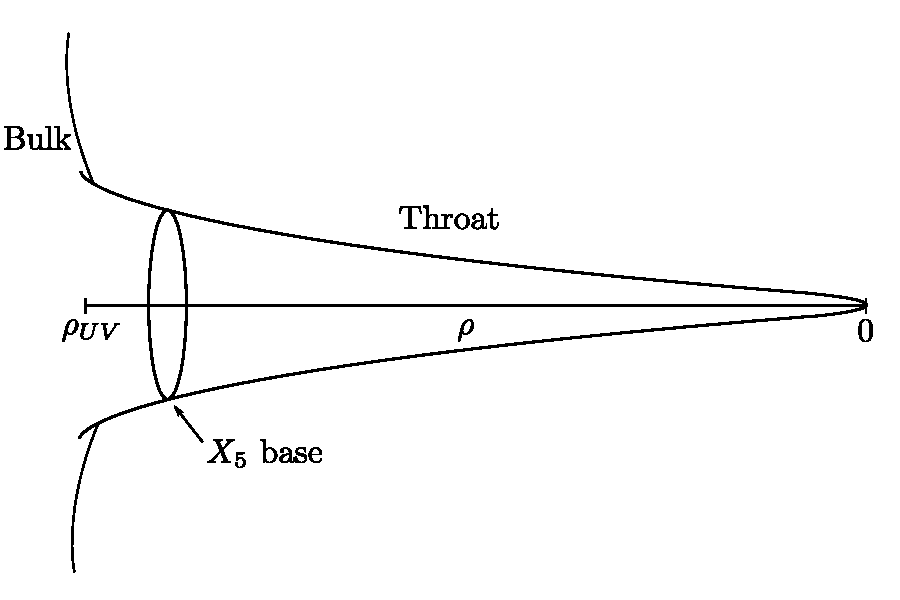
\includegraphics[width=\textwidth]{./dbi/graphs/throat-geom.pdf}
 % throat-geom.pdf: 432x288 pixel, 72dpi, 15.24x10.16 cm, bb=0 0 432 288
 \caption[Warped Throat Geometry]{Geometry of the warped throat. The radial
coordinate $\rho$ is measured from the tip of the throat to $\rho_{UV}$ at the join
with the bulk manifold.}
 \label{fig:throat-geom}
\end{figure}

% 

If one assumes that the bulk volume is 
non-negligible relative to 
that of the throat ($V_{6\,\mathrm{throat}} < V_{6}$), 
it follows that $\Mpl^2> V_{6\,\mathrm{throat}}\kappa_{10}^{-2}$. 
For a warped $AdS_5 \times X_5$ geometry, this leads to an 
upper limit on the total variation of the inflaton field in 
the throat region in terms of the D3 charge:
% 
\begin{equation}
\label{eq:BMbound-dbi}
\frac{\varphi_{UV}}{\Mpl}   < \frac{2}{\sqrt{N}} \,.
\end{equation}
% 


Condition (\ref{eq:BMbound-dbi}) may be converted into a 
corresponding limit on the tensor-scalar ratio by noting from 
the definition (\ref{eq:epsdefn-dbiintro})
that $\dot{\varphi}^2 /\Mpl^2 = 2\varepsilon_H H^2/P_{,X}$.
This implies that the variation of the inflaton field 
is given by the Lyth bound \eqref{eq:genlyth-dbiintro} 
\cite{lyth,bmpaper}:
% 
\begin{equation}
\label{eq:rtheory}
\frac{1}{\Mpl^2} \left( \frac{\d\varphi}{\d \N} \right)^2 =
\frac{r}{8} \,,
\end{equation}
% 
where $\N$ is the number of e-foldings as defined in \eq{eq:nefolddefn-intro}. 
Since $\vp_*$, the field value during observable inflation,  is
less than $\varphi_{UV}$,
this results in an upper bound on the observable tensor-scalar ratio
\cite{bmpaper}: 
% 
\begin{equation}
\label{eq:BMboundr}
r_*  < \frac{32}{N (\Neff)^2} \,.
\end{equation}
% 
The effective number of e-foldings, $\Neff$, defined in
\eq{eq:Neff-dbiintro}, 
is a model-dependent parameter that quantifies 
how $r$ varies during the final stages of inflation. Since $\cs\PX = 1$ in the
standard DBI model, 
it follows that $\Neff = \N_\mathrm{end}$ if $r$ is constant during inflation,
where $\N_\mathrm{end}$ is the total number of e-foldings
from the epoch of observable inflation until inflation ends.


Typically, one expects $30 \lesssim {\Neff} \lesssim 60$, 
although smaller values may be possible if the slow roll conditions are 
violated after observable scales have crossed the horizon. 
Furthermore, $N \gg 1$ is necessary 
for backreaction effects to be negligible \cite{bmpaper}. 
Hence, the constraint \eqref{eq:BMboundr} 
imposes a strong restriction on DBI inflationary models. 
On the other hand, the numerical value 
of $\Neff$ is uncertain.  
Our aim here is to focus on the range of values covered by the 
inflaton field during the observable stages of inflation. 
This will result in a constraint on the tensor modes that 
can be expressed in terms of observable parameters.  


To proceed, we denote the change in the value of the inflaton field over 
observable scales by 
$\Delta  \varphi _{*} = \sqrt{T_3} \Delta \rho_{*}$. 
Since the brane moves towards the tip of the throat in 
UV DBI inflation, it follows that $\rho_{*} > \rho_{end} >0$, which 
implies that  
% 
\begin{equation}
\label{eq:importantbound}
\rho_{*} > |\Delta \rho _{*}| \,.
\end{equation}
% 
This change in the inflaton value will correspond 
to a fraction of the throat volume, 
$| \Delta V _{6\,*}|  < {V_{6\,\mathrm{throat}}} \lesssim {V_6} $,
where equality in the second limit arises if
the bulk volume is negligible. Hence, 
$| \Delta \varphi_* |$ is bounded such that  
% 
\begin{equation}
\label{eq:halfwayconstraint}
\left( \frac{\Delta \varphi}{\Mpl} \right)^2_{*} < 
\frac{T_3 \kappa_{10}^2 (\Delta \rho_{*})^2}{|\Delta V_{6\,*}|} \,.
\end{equation}
%  


The observations of the CMB 
that directly constrain the primordial tensor perturbations only 
cover multipole values in the range $2 \le l \lesssim 100$. 
This is equivalent to ${\Delta \N_{*}} \simeq {4}$ 
e-foldings of inflationary expansion and, in general,   
corresponds to a narrow range of inflaton values. 
To a first approximation, therefore, the fraction of the throat volume 
(\ref{eq:throatvolume}) that is accessible to cosmological 
observation can be estimated to be 
% 
\begin{equation}
\label{eq:trapezium}
| \Delta V_{6\,*} | \simeq \mathrm{Vol}(X_5) 
\frac{|\Delta \rho_*| \rho^5_{*}}{h^{4}_{*}} \,.
\end{equation}
% 
Combining the inequality (\ref{eq:importantbound}) with \eq{eq:trapezium} 
then implies that 
% 
\begin{equation}
\label{eq:trapeziumlimit}
|\Delta V _{6\,*}| > \mathrm{Vol}(X_5) 
\frac{(\Delta \rho_* )^6}{h^{4}_*}  \,.
\end{equation}
% 
Substituting the condition \eqref{eq:trapeziumlimit} into the bound
\eqref{eq:halfwayconstraint} gives
\begin{equation}
\label{eq:hbound6}
\left( \frac{\Delta \varphi}{\Mpl} \right)_*^6 < \frac{\pi T_3}{\Vol} 
\left( \frac{h_*}{\Mpl} \right)^4 \,,
\end{equation}   
and using $T(\vp) = T_3 h^4$ and 
\eq{eq:obswarp-dbiintro} yields the upper limit
% 
\begin{equation}
\label{eq:boundpower6}
\left( \frac{\Delta \varphi}{\Mpl} \right)^6_{*} 
< \frac{\pi^3}{16\mathrm{Vol}(X_5)} r^2 \Pr 
\left( 1- \frac{1}{3\fnleq} \right)  \,.
\end{equation}
% 
Hence, employing the Lyth bound \eqref{eq:rtheory} in the form
$(\Delta \varphi_* / \Mpl )^2 \simeq 
r (\Delta \N_*)^2 /8$  
results in a very general upper limit on the tensor-scalar ratio: 
% 
\begin{equation}
\label{eq:generalbound}
r_{*} < \frac{32 \pi^3}{(\Delta \N_*)^6 \mathrm{Vol}(X_5)} 
\Pr \left( 1- \frac{1}{3\fnleq} \right) \,.
\end{equation}
% 


Condition (\ref{eq:generalbound}) is 
only weakly dependent on the level of non-Gaussianity 
when $-\fnleq > 5$ and we may therefore neglect the 
factor involving this parameter. 
Substituting the WMAP5 normalisation 
$\Pr \simeq 2.5 \times 10^{-9}$ then implies that
%  
\begin{equation}
\label{eq:upperbound}
r_{*} < \frac{2.5\times 10^{-6}}{( \Delta \N_*)^6 \mathrm{Vol}(X_5)} \,.
\end{equation}
% 
Furthermore, the most optimistic 
estimate for the minimum number of e-foldings that could be 
probed by observation is $\Delta \N_{*} \simeq 1$, whereas
a generic compactification arises when 
the volume of the Einstein five-manifold is $\mathrm{Vol}(X_5) 
\simeq {\cal{O}} (\pi^3)$ \cite{ks}. This yields a model-independent 
upper bound on the tensor-scalar ratio for standard UV DBI inflation:
%    
\begin{equation}
\label{eq:standardbound}
r_* < 10^{-7} \,.
\end{equation}
% 
The bound \eqref{eq:standardbound} is the main result of this section.
This value of $r$ is significantly below the sensitivity 
of future CMB polarisation experiments, which will measure 
${r} \gtrsim 10^{-4}$ \cite{Baumann:2008aq,vpj}. 
If CMB  
observations are able to span the full range of e-foldings such that
$\Delta \N_* \simeq 4$, this constraint is strengthened to 
${r_*} \lesssim {2 \times 10^{-11}}$.


Before concluding this section, we should explicitly outline all the assumptions that have lead to
\eq{eq:standardbound}. First, we are considering the relativistic limit where $\cs\ll1$. We are
also restricting ourselves to considering the UV scenario where a brane moves towards the tip of
the throat. This ensures that \eq{eq:importantbound} is satisfied. For the Lyth bound to take the
form in \eq{eq:approxlyth-dbiintro}, we have assumed that $r$ varies slowly during the observable
period of inflation. This is justified as the change in $r$ can be written in terms of the
quasi deSitter parameters $\epsilon_H, \eta_H$ and $s$ and we have assumed their magnitudes are
much less than unity.

The estimate (\ref{eq:trapezium}) was derived under the assumption  
that the integrand in \eq{eq:throatvolume}  
is constant. This inevitably introduces errors into the bound
(\ref{eq:generalbound}). However, the two limiting cases of interest 
in KS-type geometries arise 
when the warp factor scales either as $h \propto \rho$
or as $h \simeq {\rm constant}$ \cite{ks,kt}. In both cases
the integral (\ref{eq:throatvolume}) can be performed analytically. 
Indeed, if we specify $h \propto \rho^{\alpha}$ for some constant $\alpha$,  
evaluate the integral from $\rho_{*}$ 
to $\rho_{*}+\Delta \rho_{*}$, and expand to second-order in a 
Taylor series, we find that  
% 
\begin{equation}
\label{eq:limits}
\Delta V_{6\,*} \simeq \mathrm{Vol}(X_5) \frac{\rho^5_{*}}{h^{4} 
(\rho_{*} )}(\Delta \rho_*) 
\left[ 1 +\frac{(5-4 \alpha )}{2} 
\frac{(\Delta \rho_*)}{\rho_{*}} \right]  \,.
\end{equation}
% 
This implies that the error in \eq{eq:trapezium} 
is no greater than 
about $3 (\Delta \rho_* / \rho_*)$ if  
$0 \le \alpha \le 1$. More generally, it follows that a similar
error will arise for {\em any} warp factor 
$h \propto \rho^{\alpha (\rho )}$, where the function 
$\alpha (\rho)$ satisfies $0 \le \alpha (\rho ) \le 1$ 
over observable scales. 
We conclude, therefore, that \eq{eq:trapezium} 
provides a sufficiently good estimate of the volume element  
for a generic warp factor\footnote{As we shall see in the following section, 
even an order of magnitude error will make little 
difference to our final conclusions.}.

In order to neglect the $\fnleq$ term in \eq{eq:boundpower6} we have assumed that $-\fnleq>5$. As
$\cs$ has been taken to be small this is expected to be the case. The volume of the Sasaki-Einstein
manifold $X_5$ is taken to be $\mathcal{O}(\pi^3)$ in keeping with the values for known solutions.
The WMAP5 normalisation of the scalar perturbation power spectrum has also been used. Finally, in
going from \eq{eq:upperbound} to the final numerical figure in \eq{eq:standardbound} the most
``optimistic'' value, $\Delta \N_*\simeq 1$, has been chosen as this leads to the least
restrictive bound on $r$.  As described above a more realistic value of $4$ would severely
constrain $r$ due to the strong dependence of \eq{eq:upperbound} on $\Delta\N_*$.
% 
% 
% 
% 
% % % % % % % % % % % % % % % % % % % % % % % % % % % % % % % % 
% =========================================================== %
% % % % % % % % % % % % % % % % % % % % % % % % % % % % % % % % 
\section{A Lower Bound on the Primordial Gravitational Waves} 
% 
\label{sec:lower-dbi}
% % % % % % % % % % % % % % % % % % % % % % % % % % % % % % % % 
% =========================================================== %
% % % % % % % % % % % % % % % % % % % % % % % % % % % % % % % % 

The analysis of the previous section 
indicates that standard versions of UV DBI inflation generate a 
tensor spectrum that is unobservably 
small. Therefore, $r=0$ can be assumed as a prior when discussing the WMAP5
data.
However, in this case the data 
disfavours a scale-invariant density spectrum at close to the $3 \sigma$ level
($2.78\sigma$)
when the running in the spectral index, $\alpha_s \equiv \d n_s/\d\ln k$, 
is negligible \cite{Komatsu:2008hk}.  
Furthermore, a blue spectral index 
is only marginally consistent with the data when $r\ne 0$ and $\alpha_s=0$. 
(The inferred upper limit is $n_s < 1.018$.)
Although the results from WMAP5 do allow for a blue spectrum if there is 
significant negative running in the spectral index, we will 
focus in this section 
on models that generate a red spectral index $n_s<1$, since these are preferred by the current
data.  


In general, the spectral index may be related to the tensor-scalar ratio. 
After differentiating \eq{eq:csdefn-dbiintro} 
with respect to coordinate time, and employing Eqs. (\ref{eq:phidot-useful}) 
and (\ref{indices}), we find that\footnotemark
% 
\begin{equation}
\label{eq:nsconstraint}
1-n_s = 4 \varepsilon_H +\frac{2s}{1-\gamma^2} \mp 
\frac{2\Mpl^2}{\gamma} \frac{T_{,\vp}|H_{,\vp}|}{TH}  \,,
\end{equation}
% 
where the minus (plus) sign corresponds to 
a brane moving down (up) the warped throat.
%  
\footnotetext{The relationship between $\dot{\vp}$ and $H_{,\vp}$ is defined in
\eq{eq:phidot-useful}. When $\dot{\vp}<0$ and the brane moves down the throat
(UV case) $H_{,\vp}>0$. Alternatively in the IR case when $\dot{\vp}>0$ we have
$H_{,\vp}<0$. In order to remove the ambiguity we rewrite \eq{eq:phidot-useful}
using $-H_{,\vp} = \mp |H_{,\vp}|$ where the minus (plus) sign corresponds to
the UV (IR) case.}
% 
The second term in \eq{eq:nsconstraint}
can be converted into observable parameters
by defining the `tilt' of the non-linearity parameter  \cite{brane14}: 
% 
\begin{equation}
\label{eq:nnl-defn-dbi}
\nnleq \equiv \frac{\d \ln |\fnleq|}{\d\ln k}\,. 
\end{equation}
% 
This implies that $s=  3 \fnleq \nnleq /[2(1-3\fnleq)]$ and     
substitution of Eqs.~(\ref{indices})--(\ref{eq:fnlcs-dbiintro}) 
into \eq{eq:nsconstraint} then yields
% 
\begin{equation}
\label{eq:obscon1}
1-n_s = \frac{r}{4} \sqrt{1-3\fnleq} + \frac{\nnleq}{1-3\fnleq}
\mp \sqrt{\frac{r}{8}} \left( \frac{T_{,\vp}}{T} \Mpl \right)_*  \,.
\end{equation}
% 


In \Rref{lidser2}, brane inflation near the tip of a KS-type 
throat was considered, where the warped brane tension asymptotes to a 
constant value. In this regime, \eq{eq:obscon1} reduces to 
the condition $r \simeq 2.3 (1-n_s)/\sqrt{-\fnleq}$ when $|\fnleq|$ is 
sufficiently large to be detectable by Planck, 
\iec $|\fnleq| > 5$. 
It then follows from the  
WMAP5 best-fit value $n_s \simeq 0.968$ and lower limit 
$\fnleq > -151$ \cite{Komatsu:2008hk} that the gravitational wave amplitude 
is bounded both from above and below such that $0.001 \lesssim r 
\lesssim 0.01$. These bounds follow from 
current WMAP5 limits on the spectral index and the 
non-linearity parameter, but do not take into account the 
field-theoretic upper bound that must be imposed 
on the variation of the inflaton field during inflation. 


More generally, in UV DBI inflation where the brane moves towards the 
tip of the throat, it is reasonable to assume 
that the warp factor decreases monotonically 
with the radial coordinate over the observable range of inflaton values, 
\iec $dh/d \rho \ge 0$. This condition is satisfied for  
$AdS_5 \times X_5$ compactifications and KS-type solutions. 
Consequently, the third term in 
\eq{eq:obscon1} will be semi-negative definite, 
which implies that 
% 
\begin{equation}
\label{eq:halfbound}
\frac{r}{4} \sqrt{1-3\fnleq} + \frac{\nnleq}{1-3\fnleq} 
> 1-n_s \,.
\end{equation}
% 

Condition (\ref{eq:halfbound}) is a consistency relation on UV DBI 
inflation in terms of observable parameters and it 
may be combined with the upper bound 
(\ref{eq:generalbound}) to confront the scenario with observations.
Firstly, let us assume that the tensor-scalar ratio is negligible. 
The WMAP5 data implies that $1-n_s > 0.026$ at $1\sigma$, and this is only 
compatible with condition (\ref{eq:halfbound}) if 
% 
\begin{equation}
\label{eq:nnlbound}
\nnleq \simeq -2s > -3 (1-n_s ) \fnleq > -0.078 \fnleq \,.
\end{equation}
% 
However, when $-\fnleq \gg 1$, this would violate the slow roll conditions
that must be satisfied for a consistent 
derivation of the perturbation spectra 
(\ref{eq:spectra-dbiintro}). For example, the conservative 
bound $|s| < 0.1$ with $1-n_s \simeq 0.05$ is violated if  
$-\fnleq > {\cal{O}} (5)$. 

In view of this, let us consider the case where the tensor 
perturbations are non-negligible. 
The magnitude of the second term in condition (\ref{eq:halfbound}) 
is suppressed by a factor of $(-\fnleq)^{3/2} \gg 1$ 
relative to the first. This is expected to 
be a significant effect in DBI inflation. 
Consequently, 
by saturating the WMAP5 limit $\fnleq > -151$, we arrive at 
a lower bound on the tensor-scalar ratio which applies   
to any model for which the ratio $|\nnleq/\fnleq|$ is 
negligible:
% 
\begin{equation}
\label{eq:lowerbound}
r_* >  \frac{4(1-n_s)}{\sqrt{-3\fnleq}} > \frac{1-n_s}{6} \,.
\end{equation}
% 
This second bound requires $r > 0.005$ for the WMAP5 best-fit value 
$1-n_s \simeq 0.032$, which is incompatible with the upper limit 
(\ref{eq:standardbound}). 


In general, therefore, it is difficult to simultaneously satisfy 
the bounds on $r$ with the WMAP5 data
in standard UV DBI inflation. There is a 
small observational window where a blue spectrum is consistent 
with the data, in which case the lower limit 
(\ref{eq:lowerbound}) does not apply. 
However, if the tensor modes are negligible,
as implied by the inequality (\ref{eq:standardbound}), the 
data strongly favours a red spectral index with $n_s < 0.974$,
and this violates the condition (\ref{eq:lowerbound}). A significant 
detection of a red spectral index requires either a 
violation of the slow roll conditions or a sufficiently 
small value for the volume of $X_5$. 
In particular, combining the limits
(\ref{eq:upperbound}) and (\ref{eq:lowerbound}) results in the condition 
% 
\begin{equation}
\label{eq:upperboundvol}
\mathrm{Vol}(X_5) < \frac{2 \times 10^{-5}}{(1-n_s) 
(\Delta \N_{*} )^6}  \,,
\end{equation}
% 
and we find that $\mathrm{Vol}(X_5) \lesssim 10^{-7}$ 
is required for typical values $1-n_s \simeq 0.05$ and 
$\Delta \N_* \simeq 4$. 
This 
is comparable to the limit on the volume derived for the special case of a 
quadratic inflaton potential \cite{bmpaper}.  

As noted in Refs.~\cite{bmpaper} and \cite{bean}, condition 
\eqref{eq:upperboundvol} may be achieved 
if $X_5$ corresponds to a $Y^{p,q}$ space. Previously only two five-dimensional Sasaki-Einstein
metrics were explicitly known, $S^5$ and $T^{1,1}$ on $S^2\times S^3$. The $Y^{p,q}$ metrics
described in \Rref{gauntlett} are a countably infinite number of Sasaki-Einstein metrics on
$S^2\times S^3$. The metrics are parametrised by the two topological numbers $p$ and $q$, which are
coprime when the $Y^{p,q}$ is topologically $S^2\times S^3$. The volume of one of these manifolds
is proportional to $1/p$. Hence by setting $q=1$ and letting $p$ become large, this volume can be
made arbitrarily small \cite{gauntlett}. On the other hand, the largest volume occurs for $p=2$,
$q=1$ giving $\mathrm{Vol}(Y^{2,1})\simeq 0.29\pi^3$. 
% 
Small volumes could also be realised 
by orbifolding the $S^2$ symmetry of a KS-type throat. 


On the other hand, 
the upper limit (\ref{eq:upperbound}) on the gravitational waves 
follows as a consequence of assuming 
the constraint (\ref{eq:importantbound}). This  
could be violated in IR versions of the scenario, where
observable scales crossed the Hubble radius when the 
brane was near the tip of the throat and $\varphi \ll \Mpl$
\cite{brane12,brane14}. 
Nonetheless, we emphasise that the upper bound (\ref{eq:upperbound})
on the tensor modes 
will also apply to any IR DBI model for which 
$|\Delta \varphi_* | < \varphi_*$.  
In view of the above discussion, 
we will proceed in the following section
to discuss a framework for generalising the DBI scenario so 
that the constraints on the tensor modes can be satisfied. 
% 
% 
% 
% 
% % % % % % % % % % % % % % % % % % % % % % % % % % % % % % % % 
% =========================================================== %
% % % % % % % % % % % % % % % % % % % % % % % % % % % % % % % % 
\section{Relaxing the Upper Bounds}
% 
\label{sec:relaxing-dbi}
% % % % % % % % % % % % % % % % % % % % % % % % % % % % % % % % 
% =========================================================== %
% % % % % % % % % % % % % % % % % % % % % % % % % % % % % % % % 
% 
In this section, we take a phenomenological 
approach and consider the following kinetic function which has a more general form than the DBI one
but still contains a square root term:
% 
\begin{equation}
\label{eq:genaction-dbi}
P= -f_A (\varphi ) \sqrt{1-f_B (\varphi ) X} -f_C (\varphi) \,,
\end{equation}
% 
where $f_i (\varphi )$ are unspecified functions of the inflaton 
field. We will assume 
implicitly that these functions have a suitable form for 
generating a successful phase of inflation.
A direct comparison with \eq{eq:Pdefn-dbiintro} 
indicates that the standard DBI action can be recovered by setting $f_A f_B =2$. This implies
that $\cs P_{,X} =1$ and greatly simplifies the form of \eq{eq:rtheory}. 
Another important property in the DBI case is that the warp factor uniquely determines 
the kinetic structure of the action, i.e., $h^4 \propto f_A \propto f_B^{-1}$.  
In view of this, it is interesting to consider whether
the gravitational wave constraints could be weakened by relaxing one 
or both of these conditions. 

% 
% \eq{eq:genaction-dbi} 
% can be transformed into a similar form to that of 
% \eq{eq:Pdefn-dbiintro} through the field redefinition 
% % 
% \begin{equation}
% \label{eq:defvarphi}
% \tilde{\varphi} \equiv \int d \varphi \sqrt{\frac{f_Af_B}{2}}  \,.
% \end{equation}
% 

We can differentiate $P(X, \vp)$ in \eq{eq:genaction-dbi} to find:
% 
\begin{align}
 \PX &= \frac{f_A f_B}{2\sqrt{1-f_B X}} \,, \\
 P_{,XX} &= \frac{f_A f_B}{2}\frac{f_B}{2(1-f_B X)^{\frac{3}{2}}} \,.
\end{align}
% 
% 
The sound speed of fluctuations in 
the inflaton, defined in \eq{eq:defcs-dbiintro}, is then given by
%  
\begin{equation}
\label{eq:cs-dbi}
\cs = \sqrt{1-f_B X} = \frac{f_Af_B}{2} \frac{1}{P_{,X}}  \,,
\end{equation}
% 
and the scalar power spectrum \eqref{eq:Ps-dbiintro} by
% 
\begin{equation}
\label{eq:spectrum-dbi}
\Pr = \frac{1}{2\pi^2}\frac{H^4}{f_Af_B\dot{\varphi}^2}  \,.
\end{equation}
% 
However, the consistency equation (\ref{eq:rdefn-dbiintro}) and 
non-Gaussianity constraint (\ref{eq:fnlcs-dbiintro}) remain unaltered 
for this more general class 
of models \cite{lidser2}. It 
follows, therefore, 
that the CMB normalisation condition (\ref{eq:obswarp-dbiintro}):
%  
\begin{equation}
\label{eq:obswarp2-dbi}
\frac{T (\varphi)}{\Mpl^4}  = 
\frac{\pi^2}{16} r^2\Pr \left( 1-\frac{1}{3\fnleq} \right) \,,
\end{equation}
% 
generalises to a constraint on the value of $f_A (\varphi_*)$:
%   
\begin{equation}
\label{eq:observef1}
\left( \frac{f_A}{\Mpl^4} \right)_{*} \simeq \frac{\pi^2}{16} r^2\Pr
\left( 1- \frac{1}{3\fnleq} \right)  \,.
\end{equation}
% 
Finally, the expression for the scalar spectral index
follows by generalising the derivation of \eq{eq:obscon1} given by
% 
\begin{equation}
\label{eq:obscon1-repeat}
1-n_s = \frac{r}{4} \sqrt{1-3\fnleq} + \frac{\nnleq}{1-3\fnleq}
\mp \sqrt{\frac{r}{8}} \left( \frac{T_{,\vp}}{T} \Mpl \right)_*  \,.
\end{equation}
% 
It 
is straightforward to show that for the more general kinetic function this expression becomes
%  
\begin{equation}
\label{eq:nsconstraintW}
1-n_s = \frac{r}{4} \sqrt{1-3\fnleq}
 +\frac{\nnleq}{1-3\fnleq} \mp \sqrt{\frac{r}{4f_A f_B}} \left( 
\frac{f_{A,\vp}}{f_A} \Mpl \right)_*  \,.
\end{equation}
% 


% \eq{eq:defvarphi} also allows us to deduce 
% that the infinitesimal variation of the effective 
% field $\tilde{\varphi}$ is given by the Lyth bound, 
% $(\Delta \tilde{\varphi} /\Mpl )^2 \simeq 
% r (\Delta \N)^2/8$. This implies that 
% the variation of the inflaton field during inflation is 
% % 
% \begin{equation}
% \label{eq:newphivar}
% \int_0^{\varphi_{*}} \frac{d\varphi}{\Mpl} \, \sqrt{\frac{f_Af_B}{2}} 
% = \sqrt{\frac{r_*}{8}}  \Neff \,.
% \end{equation}
% % 

\subsection{A More General BM Bound}

The BM bound \eqref{eq:BMboundr} restricts the maximal 
variation of the scalar field $\varphi$ in the full throat region for DBI inflation. 
This is determined by expression \eqref{eq:BMbound-dbi} 
for generic warped geometries that are asymptotically 
$AdS_5 \times X_5$ away from the tip of the throat. However, in Section~\ref{sec:lyth-dbiintro} the
Lyth bound was also defined for general
non-canonical actions. For the more general kinetic function
\eqref{eq:genaction-dbi}, the BM bound becomes
% 
\begin{equation}
\label{eq:bmboundgen-dbi}
 r < \frac{32}{N(\Neff)^2}\cs\PX = \frac{16}{N(\Neff)^2}f_A f_B \,.
\end{equation}
% 
To use this bound we must be able to calculate $\Neff$ over the full range of e-foldings of
inflation. This requires knowledge of the behaviour of $f_A$ and $f_B$ over that range. 

A more cautious approach would be to restrict our attention to 
the observable stage of inflation.
Assuming that the variation
of $f_Af_B = 2 \cs\PX$ is negligible during that epoch, we can use
\eq{eq:approxlyth-dbiintro} which states that 
% 
\begin{equation}
\label{eq:genphivary1}
\left( \frac{\Delta \varphi}{\Mpl} \right)^2_{*} \simeq 
\frac{(\Delta \N_{*} )^2}{8} \left(\frac{r}{\cs\PX}\right)_*  
= \frac{(\Delta \N_{*} )^2}{4} \left(\frac{r}{f_A f_B}\right)_*  \,.
\end{equation}
% 
In addition, 
if observable scales leave the horizon 
while the brane is inside the throat, the change in the field value 
must satisfy $| \Delta \varphi_*|<\varphi_{UV}$. It follows from \eqs{eq:bmboundgen-dbi} and
\eqref{eq:genphivary1}, therefore, that 
% 
\begin{equation}
\label{eq:genBMbound}
r_*< \frac{32}{N (\Delta \N_{*})^2} (\cs\PX)_* = \frac{16}{N (\Delta \N_{*})^2}
(f_Af_B)_* \,.
\end{equation}
% 

Condition 
(\ref{eq:genBMbound}) will be referred to as the 
generalised BM bound. 
We have been
conservative by restricting our discussion to the 
observable phase of inflation. A stronger condition is obtained by using
\eq{eq:bmboundgen-dbi}, which is equivalent to substituting $\Delta \N_* \rightarrow 
\Neff$. If 
$f_Af_B$ remains nearly constant over the last $\N$ 
e-foldings of inflation, 
then $\Neff$ may be as large as $60$ and the right hand side of \eq{eq:genBMbound} will be reduced
by a factor of $225$. 
Thus, the generalised bound 
(\ref{eq:genBMbound}) should be regarded as a necessary 
(but not sufficient) condition to be satisfied by the tensor modes.



Given expressions (\ref{eq:observef1}) and (\ref{eq:genBMbound})
we can either constrain $r$ using a specified value for $f_B$, or find a necessary
condition on the value of $f_B(\varphi_*)$
for the generalised BM bound to be satisfied using $r$ and $\Pr$:
%  
\begin{equation}
\label{eq:f2bound}
\frac{f_B (\varphi_*)\Mpl^4}{N} > \frac{(\Delta \N_*)^2}{\pi^2} 
\frac{1}{r\Pr} \,.
\end{equation}
% 


In UV models, identical arguments that led to 
the lower limit (\ref{eq:lowerbound}) on the tensor-scalar ratio
will also apply in this more general context if, as expected, $f_A (\varphi) $ 
is a monotonically increasing function. 

A necessary condition for
the lower and upper limits
(\ref{eq:lowerbound}) and (\ref{eq:genBMbound}) to be compatible, therefore, is  
that  
% 
\begin{equation}
\label{eq:evade}
f_Af_B > \frac{N (\Delta \N_*)^2 (1-n_s)}{4\sqrt{-3\fnleq}} \,.
\end{equation}
% 


In IR scenarios, however, the positive sign will apply in the 
last term of the right-hand side of \eq{eq:nsconstraintW}.
Hence, assuming $f_{A,\vp} >0$ and neglecting the term proportional to 
$\nnleq/\fnleq$ yields another {\em upper} limit on the tensor-scalar ratio:
% 
\begin{equation}
\label{eq:IRupper}
r_* < \frac{4(1-n_s)}{\sqrt{-3\fnleq}}  \,.
\end{equation}
% 
Combining conditions (\ref{eq:f2bound}) and (\ref{eq:IRupper}) 
therefore leads to a constraint on $f_B (\varphi_*) $
for the generalised BM bound to be satisfied in IR inflation: 
% 
\begin{equation}
\label{eq:f2IRlower}
\frac{f_B\Mpl^4}{N} > \frac{(\Delta \N_*)^2}{4\pi^2}
\frac{\sqrt{-3\fnleq}}{(1-n_s)\Pr}  \,.
\end{equation}
% 

To summarise, for the more general kinetic function in \eq{eq:genaction-dbi}, the parameters
$f_A$ and $f_B$ must satisfy \eqs{eq:observef1} and \eqref{eq:f2bound}, where we have restricted our
interest to the era of observable inflation. For UV models the lower and upper bounds on the
tensor-scalar ratio will be compatible if \eq{eq:evade} is satisfied. For IR models two upper
bounds on $r$ have been found, which when combined constrain $f_B$ as in \eq{eq:f2IRlower}. This
constraint will prove useful in Section~\ref{sec:ir-largen-bound-multi}.

\subsection{The New Upper Bound for General Models}

The newly derived upper bound on $r$ for DBI models, \eq{eq:generalbound}, arises 
because the warp factor in standard DBI models 
completely specifies the kinetic 
energy of the inflaton field. Deriving a corresponding bound for 
the generalised model (\ref{eq:genaction-dbi}) would be more involved, 
since the CMB normalisation (\ref{eq:observef1}) only 
directly constrains the function 
$f_A (\varphi )$ and this may not necessarily depend on the warp factor. 
Instead, the constraint \eqref{eq:hbound6}, given by
% 
\begin{equation}
\label{eq:hbound6-repeat-dbi}
\left( \frac{\Delta \varphi}{\Mpl} \right)_*^6 < \frac{\pi T_3}{\Vol} 
\left( \frac{h_*}{\Mpl} \right)^4 \,,
\end{equation} 
% 
can be 
combined with \eq{eq:genphivary1} to derive a limit 
on the tensor-scalar ratio in terms of the warp factor and $P(X,\vp)$. We find
that 
% 
\begin{equation}
\label{eq:LHbound}
r_* < \frac{8}{(\Delta \N)_*^2} \left(\frac{\pi T_3}{\Vol} \right)^{1/3} 
\left( \frac{h_*}{\Mpl} \right)^{4/3} \left( \cs P_{,X} \right)_* \,.
\end{equation}
% 
This bound is valid for any $P(X,\vp)$ in the warped throat including the
generalised DBI function given in \eq{eq:genaction-dbi}.
For a specific model where the warp factor and 
the functions $f_i (\varphi )$ are determined by particle 
physics considerations,   
condition \eqref{eq:LHbound} 
may be interpreted as a bound that relates 
the tensor modes directly to the value of the inflaton field during observable 
inflation. This constraint provides a consistency 
check that any given model must satisfy 
irrespective of the form of the inflaton potential. 
% 

It is worthwhile to compare \eq{eq:LHbound} with the BM bound for the full evolution given in
\eq{eq:bmboundgen-dbi}. To evaluate the BM bound requires knowledge of $f_A$ and $f_B$ over the
whole of the inflationary era. 
In contrast, using \eq{eq:LHbound} only requires values during observable inflation. However
$\cs\PX=f_A f_B/2$ must be assumed to be slowly varying for \eq{eq:LHbound} to
be valid. As discussed in Section~\ref{sec:lyth-dbiintro} this is a reasonable assumption for
models in which $\PX$ is larger than $\mathcal{O}(\epsilon_H^2)$ during observable inflation. 

As the two bounds provide upper limits on $r$ their relative strength can be compared. The bound
\eqref{eq:LHbound} is stronger than the full throat BM bound if
% 
\begin{equation}
\label{eq:LHstronger}
h_*^{4/3}N < 20 \left( \Vol \gs \right)^{1/3}  
\left( \frac{\ms}{\Mpl} \right)^{-4/3} 
\frac{( \Delta \N )_*^2}{\Neff^2} \,.
\end{equation}
% 
For typical field-theoretic values $\Vol \simeq \mathcal{O}(\pi^3)$, $\ms \simeq
0.1 \Mpl$ 
and  $\gs \simeq 10^{-2}$, this implies that
%  
\begin{equation}
\label{eq:LHstronger1}
h_*^{4/3} N < 300 \frac{(\Delta \N)^2_*}{\Neff^2} \,.
\end{equation}
% 
If the more conservative approach outlined above is taken, the BM bound for observable
inflation, \eq{eq:genBMbound}, is weaker than \eq{eq:LHbound} when
% 
\begin{equation}
\label{eq:LHstronger-weakBM}
h_*^{4/3} N < 300 \,.
\end{equation}
% 

To summarise this section, new bounds have been derived which generalise those described in
Section~\ref{sec:upper-dbi} to the case of the kinetic function in \eq{eq:genaction-dbi}.
The expressions \eqref{eq:bmboundgen-dbi}, \eqref{eq:genBMbound} and \eqref{eq:LHbound} imply that
the 
bounds on $r$
could be relaxed if $2\cs\PX = f_Af_B \gg 1$ on observable scales. 
It is therefore important to develop string-inspired models 
where this condition arises naturally. We will explore this possibility in the
next chapter.


% 
% 
% 
% % % % % % % % % % % % % % % % % % % % % % % % % % % % % % % % 
% =========================================================== %
\section{Review of Other DBI Based Models} 

\label{sec:others-dbi}
% =========================================================== %
% % % % % % % % % % % % % % % % % % % % % % % % % % % % % % % % 
\begin{figure}[htbp]
 \centering
 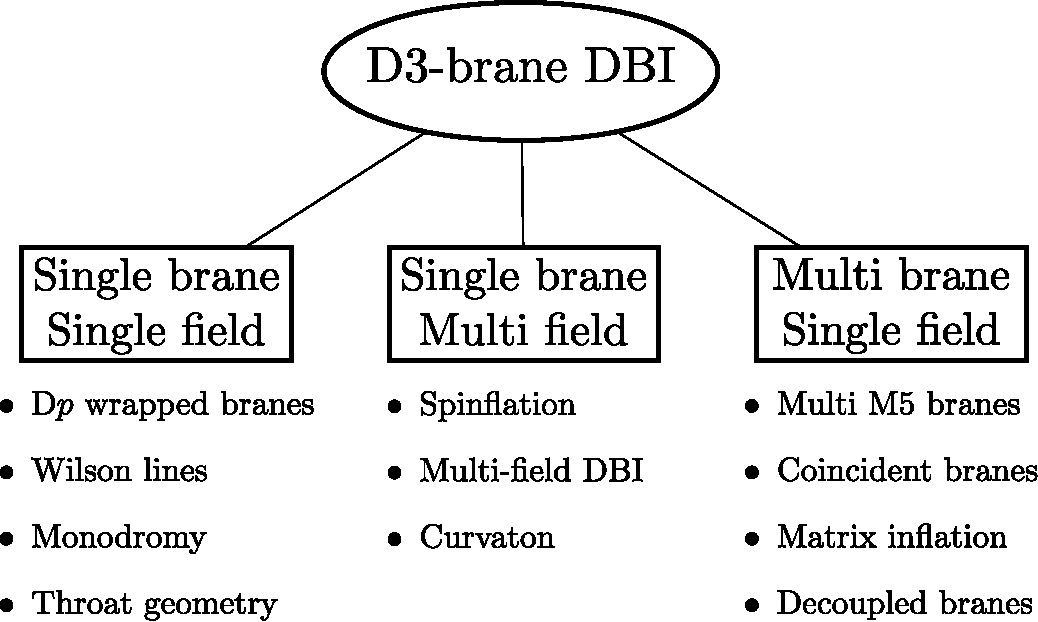
\includegraphics[width=0.8\textwidth]{./dbi/graphs/dbi-review.pdf}
 % dbi-review.pdf: 498x327 pixel, 72dpi, 17.57x11.54 cm, bb=0 0 498 327
 \caption[Recent DBI Inspired Models]{A schematic of recent DBI inspired models}
 \label{fig:review-dbi}
\end{figure}
% 

We have found that the standard DBI model appears to be in conflict with
observations. Many attempts have since been made to modify the original scenario in
order to evade the bounds derived above. These new models can be classified according
to
whether they involve single or multiple fields and single or multiple branes.
Figure~\ref{fig:review-dbi} lists some of the models in
each category.


The most straightforward extensions of the DBI model are single field, single brane
models. 
These have a single degree of freedom, as in the D3-brane model, but
they rely on other physical mechanisms to ease the bounds on $r$.
A natural extension to the single ${\rm D3}$-brane model 
is to consider a ${\rm D}p$-brane wrapped around a $(p-3)$-cycle of the 
internal space.
This leads to a change in the relationship
between $\rho$ and $\vp$ from that defined in Section~\ref{sec:dbiinflation}
\cite{Kobayashi:2007hm, Becker:2007ui, Ward:2007gs}.  
For example, Becker \etal \cite{Becker:2007ui} 
have proposed a model in which inflation is driven by a wrapped ${\rm D5}$-brane. 
In this case, the range of allowed values for the inflaton 
becomes independent of the throat charge, $N$, which weakens the upper bound on 
the tensor-scalar ratio to $r \lesssim 0.04$. (Strictly speaking there is a weak
dependence on the charge since $\Delta \varphi \sim N^{-1/4}$.)
However, in arriving at this bound, it was assumed that 
backreaction effects of any fluxes in the throat were 
negligible. 
Kobayashi \etal \cite{Kobayashi:2007hm} 
considered both ${\rm D5}$ and
${\rm D7}$ wrapped brane models, but concluded that the former case
required an excessively large background charge in 
order to relax the bounds on $r$. 
% 
This requirement is highly constraining, but is
still not as restrictive as the value of the charge required by the single brane scenario,
which effectively rules this model out. 
% 
Thus, a wrapped brane configuration is preferable to
the single D3-brane model, but the parameter space of the former is still severely
limited by the WMAP5 observations \cite{Alabidi:2008ej}. 
% However
% the difficulty in these models is that the backreaction is no longer under
% control. 


Another interesting proposal is warped Wilson line DBI. In this scenario, moduli
fields associated with Wilson
lines play the role of the inflaton \cite{Avgoustidis:2008zu}. This scenario is
T-dual to the
standard DBI model with non-parallel branes. In general, the model describes the
physics of a single brane with multiple position fields and multiple Wilson line
fields.
% 
In \Rref{Avgoustidis:2008zu}, observational predictions were derived for
the case when the brane position is fixed and only one Wilson line degree of freedom
is used. This implementation is therefore a single brane, single field model.
% 
By following the method outlined in Section~\ref{sec:upper-dbi} for this single field model,
a lower bound on $r$ was derived, instead of the upper bound \eqref{eq:upperbound}
\cite{Avgoustidis:2008zu}. The lower bound \eqref{eq:lowerbound} remains valid for
this scenario. 
% 
There are, therefore, two lower bounds on $r$ and the inconsistency of the
standard DBI model is not replicated. 
 


Changing the physical setting can also allow larger field ranges, which in turn can relax the
bounds on $r$. One such example is the case of a D4-brane in compactified manifolds
containing monodromies. 
The large field variations in this single brane, single field model lead to possibly
observable
tensor modes
\cite{Silverstein:2008sg}. Although formulated in Type IIA string theory, the
monodromy scenario has a simple inflationary interpretation as a large field, slow roll
model with a potential $V(\vp)\propto\vp^{2/3}$. 

The tensor-scalar ratio and other observable quantities are
significantly altered if the throat geometry is not of the $AdS_5$ type, even in the case of the
standard D3-brane model \cite{Gmeiner:2007uw}. In
\Rref{Butti:2004pk}, a one parameter family of solutions was found, which interpolates
between the
Klebanov-Strassler (KS) \cite{ks} and Maldacena-Nu\~{n}ez
\cite{Maldacena:2000yy} throats. As the throat geometry moves away from KS, more
non-Gaussianity is produced whereas the tensor-scalar ratio is reduced.
The choice of throat geometry, therefore, could affect the bounds on $r$
and must be considered when models are compared.



The next class of models that can be investigated are the single brane, multi-field
configurations. 
% 
The warped throat is six-dimensional, so it is natural to consider cases where
the D3-brane is not restricted to a radial trajectory. This was investigated in
Refs.~\cite{spinflation} and \cite{Huang:2007hh}. Increasing the degrees of
freedom in this way introduces the possibility of entropy mode production. There are also
changes in the predictions for the amount and type of non-Gaussianity produced
and the constraints on $r$ can be eased \cite{Arroja:2008yy, Langlois:2009ej,
Langlois:2008qf, Langlois:2008wt, Mizuno:2009mv, Mizuno:2009cv, RenauxPetel:2009sj}.
%
The bounds on $r$ could also be affected if a non-negligible part of the
curvature perturbation was produced by a curvaton field \cite{Lyth:2001nq}.
Curvaton fields arise generically in scenarios containing warped throats,
particularly for propagation near the tip \cite{Li:2008fm, Kobayashi:2009cm}. 
% 
% Differences in
% the bi- and tri-spectra could enable multi-field DBI models to be distinguished
% from single field ones. In particular multi-field DBI models
% have a unique tri-spectrum term with amplitude proportional to $\fnlloc\fnleq$
% \cite{RenauxPetel:2009sj}. This opens the possibility of a distinct
% observational signature for this type of model.
% 

Investigations have also been made into models with multiple branes, each of which
has a single dynamical field. In Refs.~\cite{Cai:2008if} and \cite{Cai:2009hw}, no
interactions between branes were considered, and the branes could conceivably propagate in different
throats. The action for $n$ decoupled branes in the
relativistic limit is the sum of $n$ copies of the DBI action
\eqref{eq:DBIaction-dbiintro}. The power spectrum of curvature perturbations is
enhanced by a factor of $n^{3/2}$ with respect to the single brane case. Consequently, the value
of the tensor-scalar ratio will be reduced. 


We have not yet addressed models with multiple branes but only one effective
degree of freedom. Multiple M5-branes in M-theory act with an effective
single degree of freedom, but the Lyth bound is now significantly weakened. Large
field ranges and an observable tensor signal are therefore possible \cite{Krause:2007jr}. 
Another proposal is that of $n$ D3-branes which are coincident and propagating in a
warped throat \cite{thomasward, hltw, Ward:2007gs, Berndsen:2009ww}. The
non-Abelian nature of the interactions between the branes differentiates this model
from other multi-brane models and the model is also known as ``Matrix Inflation''.
In Chapter~\ref{ch:multibrane} we
investigate this model in the relativistic limit
for both large and small $n$, and show how the constraints derived in this
chapter can be applied.


% 
% 
% 
% % % % % % % % % % % % % % % % % % % % % % % % % % % % % % % % 
% =========================================================== %
\section{Discussion}
\label{sec:conclusion-dbi}
% =========================================================== %
% % % % % % % % % % % % % % % % % % % % % % % % % % % % % % % % 

In this chapter, we have derived an upper limit on
the amplitude of the primordial gravitational wave spectrum
generated during UV DBI inflation. We considered   
the maximal inflaton field variation   
that can occur during the observable stages of inflation and assumed  
only that the brane was propagating inside the throat during that epoch. 
The bound (\ref{eq:upperbound}) is valid for an arbitrary inflaton potential and 
warp factor (modulo some weak caveats) and can be expressed 
entirely in terms of observable parameters, once the volume of 
the five-dimensional sub-manifold of the throat has been specified. 
The inferred upper limit on $r$ is surprisingly strong. 
We find that the standard UV  
scenario predicts tensor perturbations that are undetectably small, 
at a level ${r_*} \lesssim {10^{-7}}$. 

The current WMAP5 data 
favours models that generate a red spectral index, $n_s<1$,
when both the gravitational waves and running in the scalar 
spectral index are negligible. For UV versions of the scenario, 
we have identified a corresponding 
lower limit on $r$ which applies in this region of 
parameter space, $r_* \gtrsim 0.1 (1-n_s)$. It is clear that 
the standard scenario 
cannot satisfy both the upper and lower bounds 
on the tensor modes for the observationally favoured value 
$1-n_s \simeq 0.03$.


The generality of our 
analysis implies that modifying either the inflaton potential 
or the form of the warp factor is unlikely to resolve this discrepancy. 
On the other hand, there are a number of possible ways of reconciling  
theory with observation. In general, 
either the upper or lower limit on $r$ needs to be relaxed. 
Weakening the latter would require a violation of the slow roll 
conditions or a blue spectral index. 
A value of $n_s >1$ is compatible with WMAP5 if the running of the 
spectral index 
is sufficiently negative, but is only marginally
consistent if just the tensor modes are non-negligible.  The 
upper limit on $r$ can be weakened by reducing 
the volume of $X_5$ or 
by generalising the DBI action. Furthermore, it need not necessarily 
apply in IR versions of the scenario, although the BM bound will still hold
in such cases. 
We considered a generalised version of the 
DBI action and identified a necessary condition on the form of such  
an action for the BM bound to be relaxed.

% As a concrete example, 
% we investigated a version of IR inflation that is driven by 
% multiple coincident branes and found that  
% the bounds on the tensor-scalar ratio can indeed 
% be made compatible if the brane charges satisfy appropriate 
% conditions.   





In conclusion therefore, we have shown that primordial gravitational wave constraints 
combined with cosmological observations of the density perturbation
spectrum act as a powerful discriminant of DBI inflationary models. 
They also serve as an important observational guide for identifying viable 
generalisations of the scenario. In Chapter~\ref{ch:multibrane} we will explore
one particular generalisation, the multi-coincident brane scenario
introduced in \Rref{thomasward}.
